% !TEX root = ../main.tex
% 本文件由 build-tex.sh 从 32-DSP指南-第32章中译.md 生成，改内容请改 md 后重新生成

\chapter{拉普拉斯变换}\label{ch-32}

信号处理的两大技术------卷积和傅里叶分析------告诉我们：一个线性系统可以完全由它的冲激响应或频率响应来理解。这是一种非常一般化的方法，因为冲激响应和频率响应几乎可以是任何形状。事实上，对科学和工程中的许多应用来说，它太一般了。我们这个宇宙中的许多参数是通过微分方程(differential
equation)相互作用的。例如，电感两端的电压正比于流过它的电流的导数；同样，施加在一个质量上的力正比于其速度的导数。物理学里充满了这类关系。这些系统的频率响应和冲激响应不能是任意的，而必须与这些微分方程的解相一致。这意味着它们的冲激响应只能由指数函数和正弦函数组成。拉普拉斯变换(Laplace
transform)就是在信号连续时分析这类特殊系统的技术。z
变换(z-transform)是离散情况下的类似技术。

\section{s 域的本质}

拉普拉斯变换是求解微分方程的一种成熟的数学技术。它以伟大的法国数学家皮埃尔-西蒙·拉普拉斯（Pierre
Simon De
Laplace，1749---1827）的名字命名。和所有变换一样，拉普拉斯变换按照一套固定的规则或公式，把一个信号变成另一个信号。如图
32-1 所示，拉普拉斯变换把时域中的信号变成 s 域(s-domain)中的信号，s
域也叫 s
平面(s-plane)。时域信号是连续的，向正负两个方向延伸到无穷，可以是周期的，也可以是非周期的。拉普拉斯变换允许时域信号是复数，但这在信号处理中很少需要。在本章的讨论以及几乎所有实际应用中，时域信号完全是实数。

如图 32-1 所示，s
域是一个复平面，即水平轴上是实数，垂直轴上是虚数。沿实轴的距离用变量
σ（小写希腊字母 sigma）表示；同样，虚轴用变量 ω 表示，即自然频率(natural
frequency)。这个坐标系允许用一对 σ 和 ω
的值来指定任何一点的位置。用复数记法，每个位置用复变量 s 表示，其中
\(s = \sigma + j\omega\)。和傅里叶变换一样，s
域中的信号用大写字母表示。例如，时域信号 x(t) 变换成 s 域信号
X(s)，也可以写成 X(σ, ω)。s 平面是连续的，向四个方向都延伸到无穷。

s
域中的每一点，除了有一个由复数定义的位置之外，还有一个复数的值。换句话说，s
平面上的每个位置都有一个实部和一个虚部。和所有复数一样，实部和虚部也可以换成幅度和相位来表示。

正如傅里叶变换用正弦波来分析信号，拉普拉斯变换用正弦波和指数函数来分析信号。从数学角度看，这使傅里叶变换成为更复杂的拉普拉斯变换的一个子集。图
32-1 用图示说明了 s 域与时域的关系。要求 s
平面上一条竖线上的值（即某个特定 σ 处的值），先把时域信号乘以指数曲线
\(e^{-\sigma t}\)。s 平面的左半边用随时间增长的指数（σ \textless{}
0）去乘时域信号，右半边用随时间衰减的指数（σ \textgreater{}
0）去乘。然后对这个经过指数加权的信号做复数傅里叶变换。得到的频谱放在 s
平面的一条竖线上：s
平面的上半部分放正频率，下半部分放负频率。要特别注意：s 平面 y 轴上（σ =
0）的值，恰好等于时域信号的傅里叶变换。

上一章讲过，复数傅里叶变换为：

\[X(\omega) = \int_{-\infty}^{\infty} x(t)\, e^{-j\omega t}\, dt\]

先把时域信号乘以指数项，就可以把它扩展成拉普拉斯变换：

\[X(\sigma, \omega) = \int_{-\infty}^{\infty} \big[x(t)\, e^{-\sigma t}\big]\, e^{-j\omega t}\, dt\]

这虽然不是拉普拉斯变换最简洁的形式，但大概是对这一技术的思路和运作方式最好的描述。为了把公式写得更短，可以把两个指数项合并：

\[X(\sigma, \omega) = \int_{-\infty}^{\infty} x(t)\, e^{-(\sigma + j\omega)t}\, dt\]

\begin{figure}[htbp]
\centering
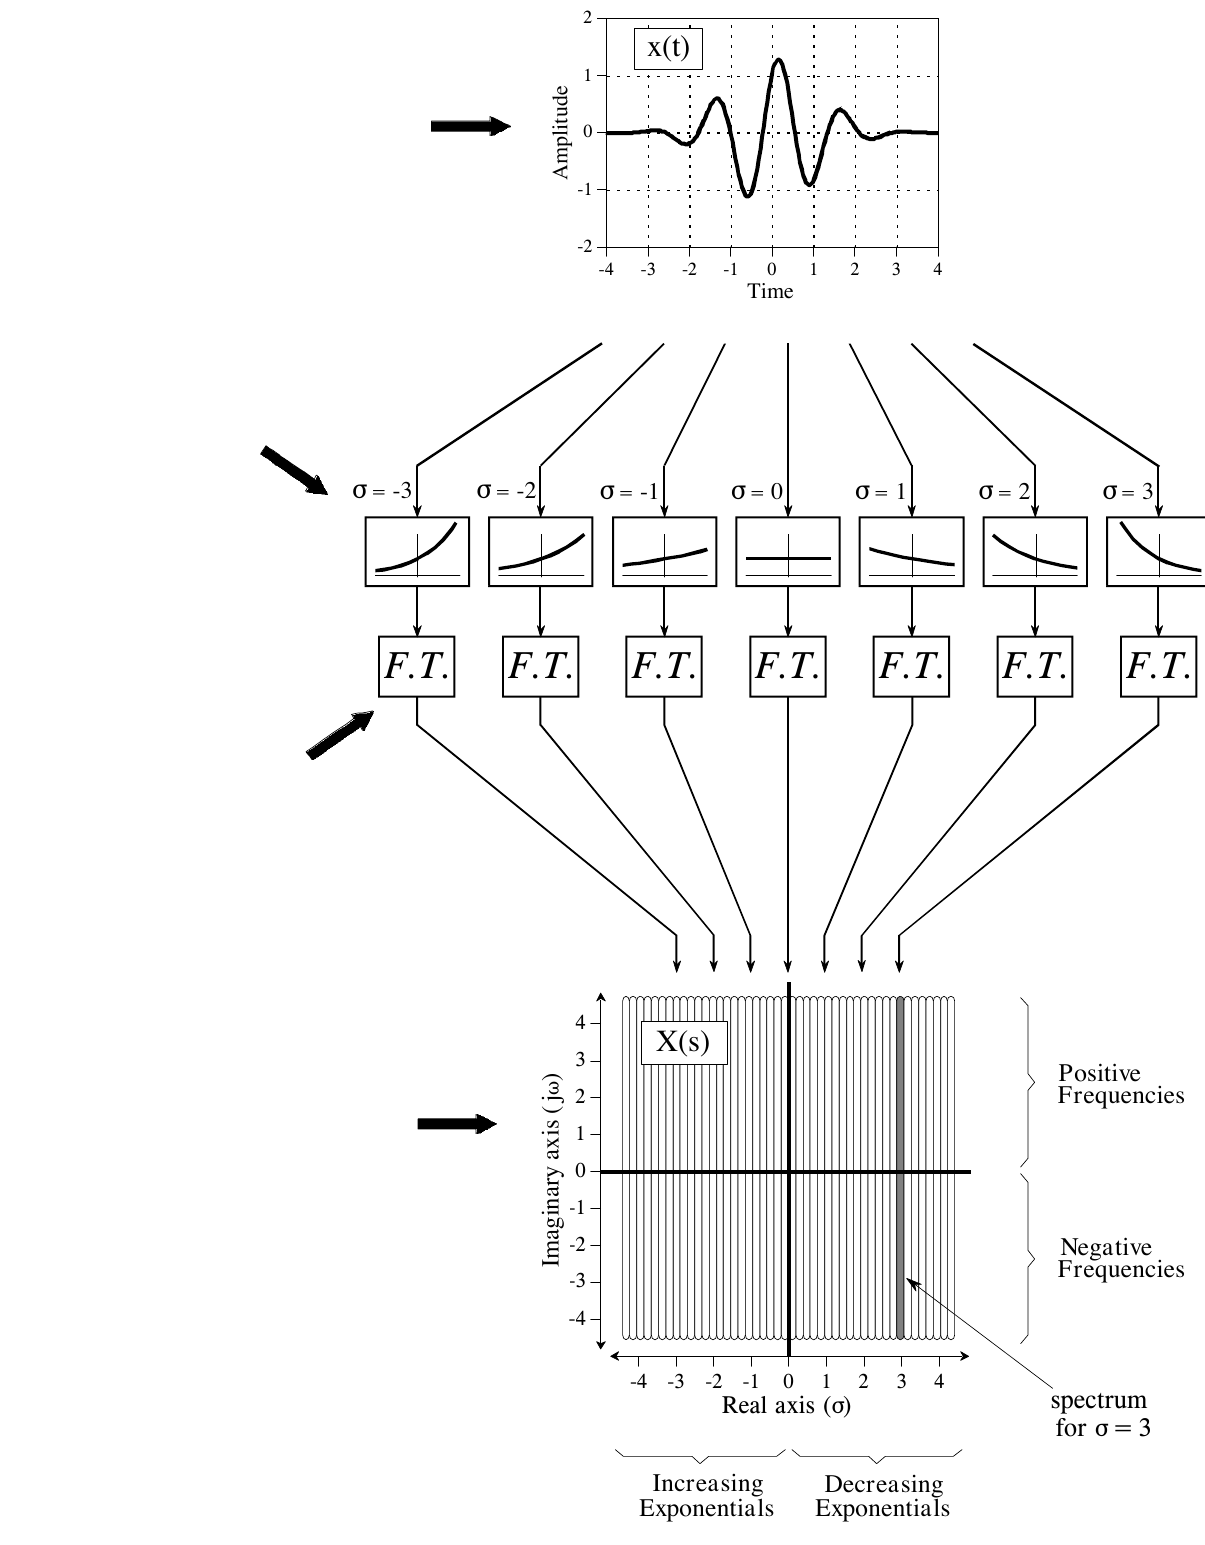
\includegraphics[width=1.000\linewidth,height=0.8\textheight,keepaspectratio]{assets/ch32/fig32-01.png}
\caption*{\textbf{图 32-1　拉普拉斯变换。} 拉普拉斯变换把时域信号 x(t) 转换成 s
域信号 X(s) 或 X(σ, ω)。s
域中每条竖线上的值，可以这样求得：把时域信号乘以衰减常数为 σ
的指数曲线，再做复数傅里叶变换。当时域信号完全是实数时，s
平面的上半部分是下半部分的镜像。原书在图左侧用四个步骤说明（图中四个箭头依次指向各步骤）：
- \textbf{第 1 步：} 从名为 x(t) 的时域信号出发。 - \textbf{第 2 步：}
把时域信号乘以无穷多条指数曲线，每条的衰减常数 σ
都不同。也就是说，对从负无穷到正无穷的每个 σ 值，计算信号
\(x(t)\,e^{-\sigma t}\)。 - \textbf{第 3 步：}
对每个经过指数加权的时域信号做复数傅里叶变换，即对从负无穷到正无穷的每个
σ 值计算
\(\int_{-\infty}^{\infty} [x(t)\,e^{-\sigma t}]\,e^{-j\omega t}\,dt\)。
- \textbf{第 4 步：} 把每个频谱排在 s 平面的一条竖线上。正频率在 s
平面的上半部分，负频率在下半部分。}
\end{figure}

（Amplitude = 幅度，Time = 时间；F.T. = 傅里叶变换；Imaginary axis (jω)
= 虚轴，Real axis (σ) = 实轴；Positive / Negative Frequencies = 正频率 /
负频率；spectrum for σ = 3 = σ = 3 处的频谱；Increasing / Decreasing
Exponentials = 增长的指数 /
衰减的指数。四段步骤说明原书排在图左侧，裁图时已去掉，译文见上。）

最后，复平面中的位置可以用复变量 s 表示，其中
\(s = \sigma + j\omega\)。这样公式就能化成更紧凑的形式：

\textbf{公式 32-1　拉普拉斯变换。} 这个公式定义了时域信号 x(t) 与 s
域信号 X(s) 之间的关系。s 域的变量 s 和 X( )
都是复数。时域信号可以是复数，但通常是实数。

\[X(s) = \int_{-\infty}^{\infty} x(t)\, e^{-st}\, dt\]

这就是拉普拉斯变换的最终形式，是信号处理和电子学中最重要的公式之一。要特别注意
\(e^{-st}\) 这一项，它叫复指数(complex
exponential)。从上面的推导可以看出，复指数是用一个表达式同时表示正弦波和指数函数的紧凑方式。

虽然我们把拉普拉斯变换解释成两个阶段的过程（先乘以指数曲线，再做傅里叶变换），但要记住，这只是一种教学手段，是把公式
32-1 拆成更简单部分的一种方式。拉普拉斯变换是联系 x(t) 和 X(s)
的单个公式，而不是一步一步的过程。公式 32-1 描述的是：如何根据 σ、ω
的值和时域信号 x(t)，计算 s 平面上的每一点（由它的 σ 值和 ω
值确定）。用傅里叶变换同时算出一条竖线上的所有点，只是为了方便，而不是必须这样做。不过，一定要记住：s
平面上沿 y 轴（σ =
0）的值恰好等于傅里叶变换。本章后面会讲到，这正是拉普拉斯变换有用的关键原因之一。

为了进一步探究公式 32-1 的本质，我们来看 s
域中的几个单独的点，考察这些位置上的值与时域信号有什么关系。首先回忆一下频域中的单个点与时域信号的关系。频域中的每个点由一个特定的
ω 值确定，对应两个正弦波：\(\cos(\omega t)\) 和
\(\sin(\omega t)\)。实部的求法是把时域信号乘以余弦波，再从 −\dspsym{∞}
积分到
\dspsym{∞}；虚部的求法相同，只是用正弦波。如果处理的是复数傅里叶变换，对应负频率
−ω 处的值，是 ω
处的值的复共轭（实部相同，虚部取负）。拉普拉斯变换只是这些概念的推广。

\begin{figure}[htbp]
\centering
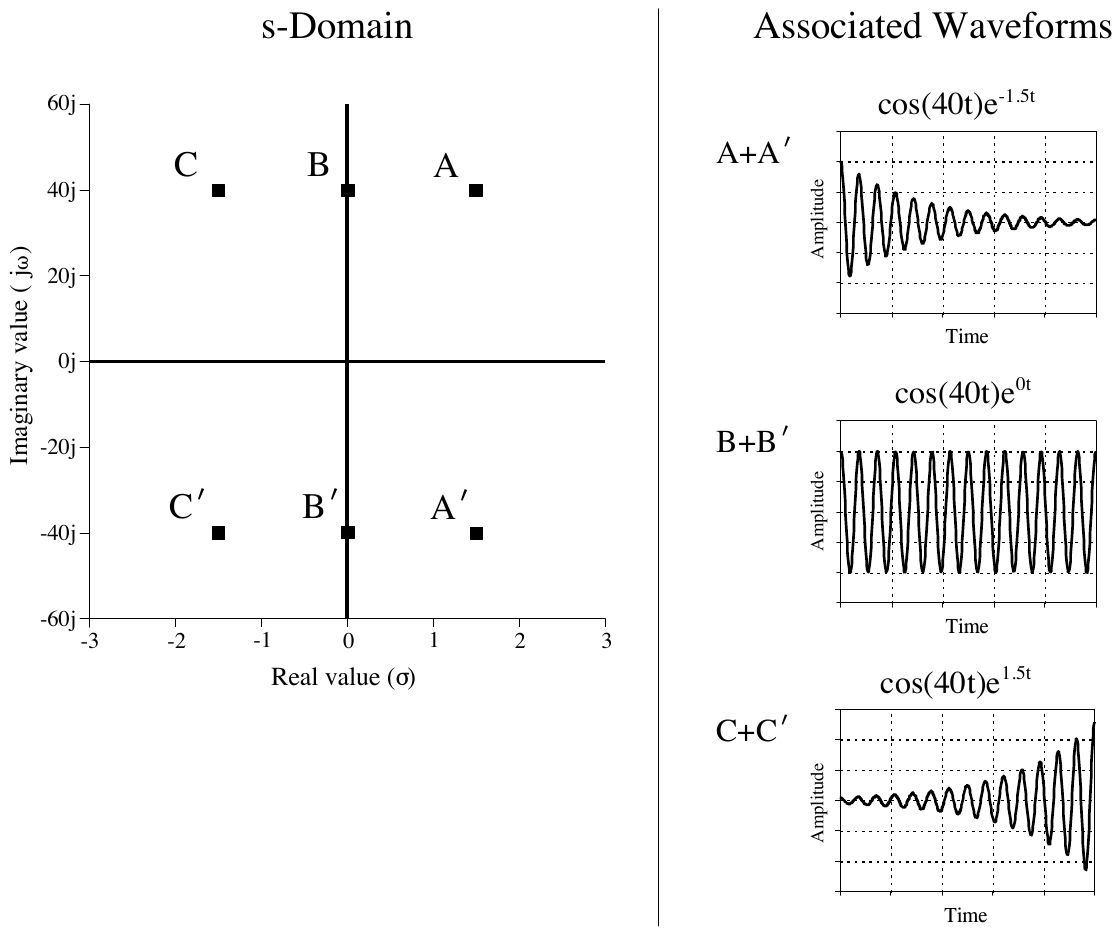
\includegraphics[width=0.933\linewidth,height=0.8\textheight,keepaspectratio]{assets/ch32/fig32-02.png}
\caption*{\textbf{图 32-2　与 s 域相关联的波形。} s
域中的每个位置由两个参数确定：σ 和
ω。这两个参数也定义了与每个位置相关联的两个波形。如果只考虑成对的点（比如
A 与 A′、B 与 B′、C 与 C′），与每个位置相关联的两个波形是频率为 ω
的正弦波和余弦波，其幅度按 σ 控制的指数规律变化。 （s-Domain = s
域，Associated Waveforms = 相关联的波形；Imaginary value (jω) =
虚部值，Real value (σ) = 实部值；Amplitude = 幅度，Time =
时间。图注原书排在左下方空白处，裁图时已去掉。）}
\end{figure}

图 32-2 给出了 s 平面上的三对点：A 与 A′、B 与 B′、C 与
C′。和复数频谱中一样，A、B、C 处的点（正频率）是 A′、B′、C′
处的点（负频率）的复共轭。s
平面的上半部分是下半部分的镜像，要对应一个实数时域信号，两半都是必需的。换句话说，把这些点成对处理就绕开了复数运算，使我们可以只用实数在时域中操作。

由于每一对点都有确定的 σ 值和 ±ω
值，每一对点都关联着两个波形：\(\cos(\omega t)\,e^{-\sigma t}\) 和
\(\sin(\omega t)\,e^{-\sigma t}\)。例如，A 与 A′ 位于 σ = 1.5、ω = ±40
处，因此对应的波形是 \(\cos(40t)\,e^{-1.5t}\) 和
\(\sin(40t)\,e^{-1.5t}\)。如图 32-2
所示，这些是幅度随时间推移按指数规律减小的正弦波。同样，与 B 与 B′
关联的正弦波和余弦波幅度恒定，因为 σ 为零。与 C 与 C′
关联的正弦波和余弦波则按指数规律增长，因为 σ 是负的。

s
平面上每个位置的值都由实部和虚部组成。实部的求法是：把时域信号乘以经过指数加权的余弦波，再从
−\dspsym{∞} 积分到
\dspsym{∞}。虚部的求法相同，只是改用经过指数加权的正弦波。以 A 与 A′
的实部为例，写成公式是：

\[\mathrm{Re}\,X(\sigma{=}1.5,\ \omega{=}\pm 40) = \int_{-\infty}^{\infty} x(t)\, \cos(40t)\, e^{-1.5t}\, dt\]

图 32-3 给出一个例子：一个时域波形、它的频谱，以及它的 s
域表示。示例时域信号是一个宽为 2、高为 1
的矩形脉冲。如图所示，这个信号的复数傅里叶变换，实部是一个 sinc
函数，虚部全为零。s
域是一个起伏的二维信号，这里用实部和虚部的地形曲面来显示。数学过程如下：

\[X(s) = \int_{-\infty}^{\infty} x(t)\, e^{-st}\, dt = \int_{-1}^{1} 1 \cdot e^{-st}\, dt\]

用文字说，我们从拉普拉斯变换的定义（公式 32-1）出发，代入 x(t) 的值
1，并把积分限改成时域信号非零部分的范围。求出这个积分，就得到用复数位置
s 和复数值 X(s) 表示的 s 域信号：

\[X(s) = \frac{e^{s} - e^{-s}}{s}\]

这虽然是最紧凑的答案形式，但复变量的使用让它难以理解，也无法画出图 32-3
那样的图。办法是把复变量 s 换成 σ + jω，再把实部和虚部分开：

\[\mathrm{Re}\,X(\sigma, \omega) = \frac{\sigma\cos(\omega)\,[e^{\sigma} - e^{-\sigma}] + \omega\sin(\omega)\,[e^{\sigma} + e^{-\sigma}]}{\sigma^2 + \omega^2}\]

\[\mathrm{Im}\,X(\sigma, \omega) = \frac{\sigma\sin(\omega)\,[e^{\sigma} + e^{-\sigma}] - \omega\cos(\omega)\,[e^{\sigma} - e^{-\sigma}]}{\sigma^2 + \omega^2}\]

\begin{figure}[htbp]
\centering
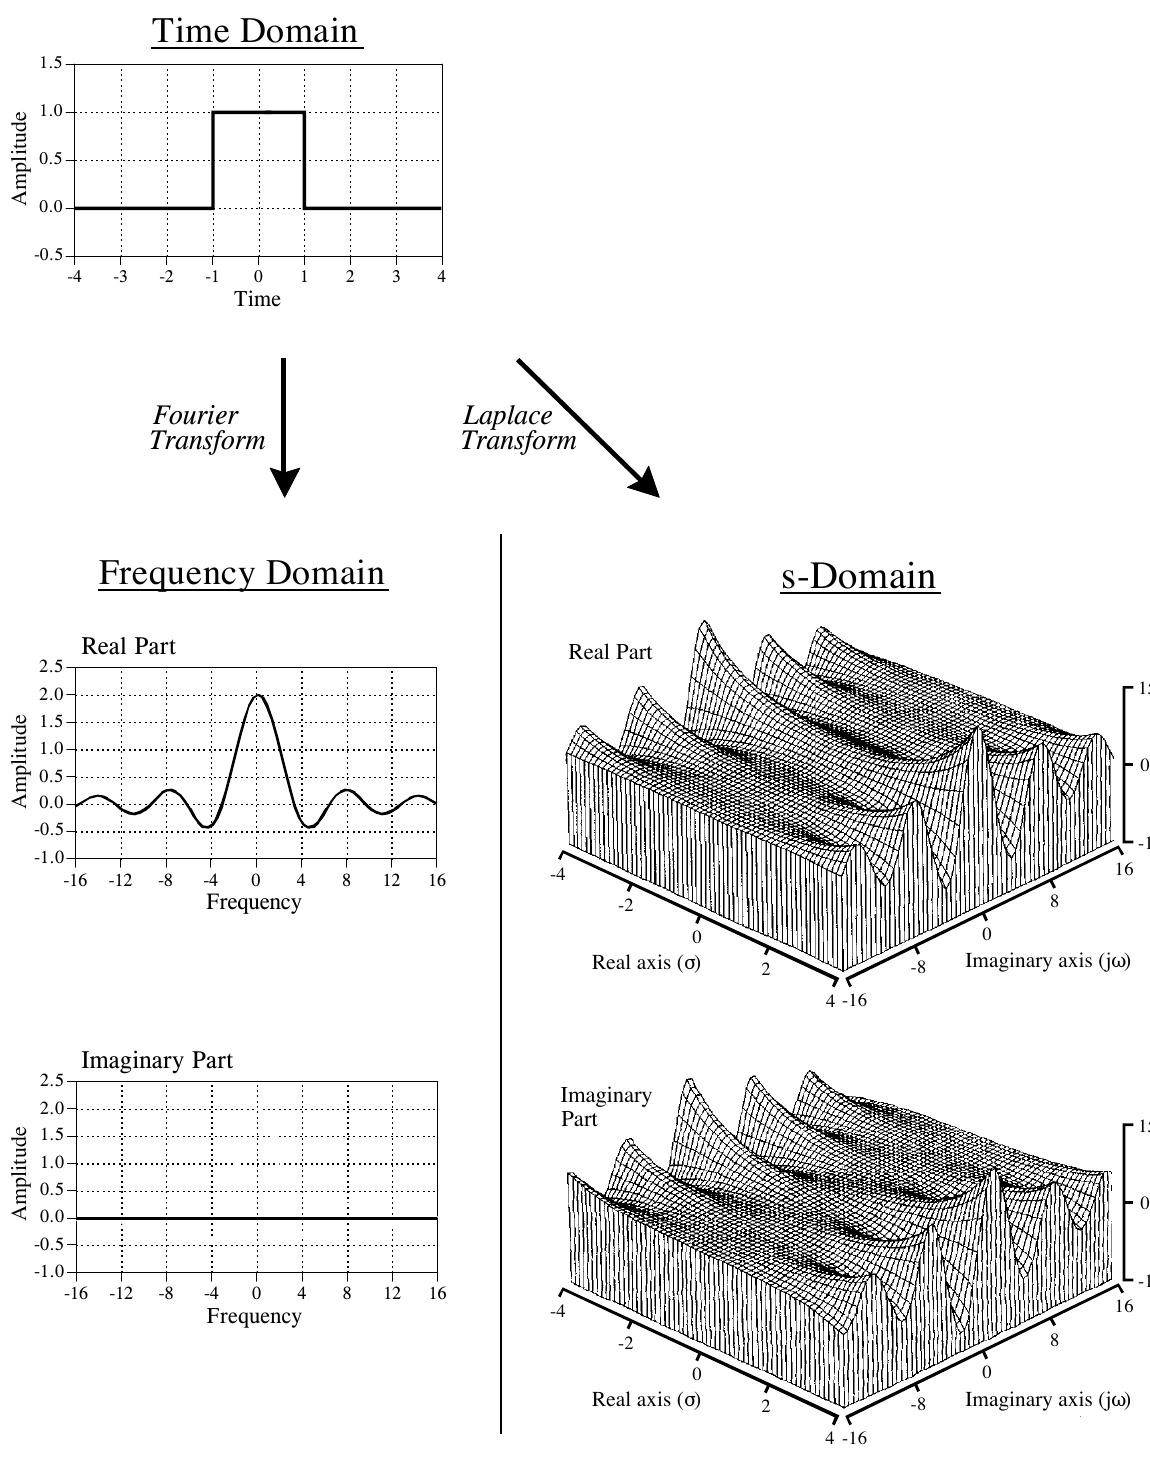
\includegraphics[width=0.958\linewidth,height=0.8\textheight,keepaspectratio]{assets/ch32/fig32-03.png}
\caption*{\textbf{图 32-3　时域、频域和 s 域。}
时域信号（矩形脉冲）用傅里叶变换变到频域，用拉普拉斯变换变到 s 域。
（Time Domain = 时域，Frequency Domain = 频域，s-Domain = s 域；Fourier
Transform = 傅里叶变换，Laplace Transform = 拉普拉斯变换；Real Part =
实部，Imaginary Part = 虚部；Amplitude = 幅度，Time = 时间，Frequency =
频率；Real axis (σ) = 实轴，Imaginary axis (jω) =
虚轴。图注原书排在右上方空白处，裁图时已去掉。）}
\end{figure}

图 32-3
中的地形曲面就是这两个公式的图像。这两个公式相当长，推导它们的数学也非常繁琐。这就带来一个实际问题：代数运算这么复杂，怎么知道我们没有算错？一种检验办法是确认这些公式在
y 轴上会化为傅里叶变换。做法是在公式中令 σ 为零，再化简：

\[\mathrm{Re}\,X(\sigma, \omega)\Big|_{\sigma=0} = \frac{2\sin(\omega)}{\omega} \qquad\qquad \mathrm{Im}\,X(\sigma, \omega)\Big|_{\sigma=0} = 0\]

如图 32-3
所示，这正是正确的频域信号，和直接对时域波形做傅里叶变换得到的结果相同。

\begin{quote}
\textbf{译注：} 上面 Re X 和 Im X 两个式子我按 \(X(s) = 2\sinh(s)/s\)
重新推了一遍：\(\sinh(\sigma + j\omega) = \sinh\sigma\cos\omega + j\cosh\sigma\sin\omega\)，再乘以
\((\sigma - j\omega)/(\sigma^2 + \omega^2)\)，得到的结果与原书完全一致。
\end{quote}

\section{拉普拉斯变换的思路}

用一个比喻来说明拉普拉斯变换在信号处理中怎样使用。想象你晚上坐火车往返于两座城市之间。地图上显示这段路线非常直，但夜色太黑，你看不到周围的任何景物。百无聊赖之下，你注意到车厢墙上有一个高度计，于是决定记录沿途的海拔变化。

几个小时后你觉得无聊，就和列车员攀谈起来：``这一带地形挺有意思，''你说，``我们的海拔似乎总体在上升，不过我注意到有几处有趣的起伏。''你不管列车员明显毫无兴趣，继续说道：``快出发时，我们经过一段陡升，紧接着又是同样陡的下降。后来又碰到一个浅浅的凹陷。''列车员担心你是个危险人物或者精神不正常，决定回应一下：``是啊，大概是这样。我们的终点在一座大山脉的山脚下，所以海拔总体在上升。另外，沿途我们会从一座大山的山脚边经过，还会穿过一个山谷的中央。''

现在想一想：你对沿线海拔与距离之间关系的理解，和列车员的理解有什么不同。由于你直接测量了沿途的海拔，你完全可以宣称自己知道这个关系的一切。相比之下，列车员也知道同样完整的信息，但形式更简单、更直观：造成路线上起伏的那些山丘和山谷的位置。你对这个信号的描述可能由成千上万个单独的测量值组成，而列车员的描述只包含几个参数。

为了说明这与信号处理的类比关系，设想我们要弄清某个电路的特性。为此，我们仔细测量了它的冲激响应和/或频率响应。前几章讲过，冲激响应和频率响应包含了这个线性系统的全部信息。然而，这并不意味着你以最简单的方式掌握了这些信息。具体地说，你把频率响应理解为一组随频率变化的数值。正如火车的比喻，频率响应可以用它周围的''地形''更容易地理解，也就是用
s 平面的特征来理解。

记住火车的比喻，回头看图 32-3，问一问：这个 s
域的形状怎样帮助我们理解频率响应？答案是：毫无帮助！这个例子中的 s
平面画出来很好看，但对于频域为什么会这样表现，它没有提供任何见解。这是因为拉普拉斯变换是为分析一类特定的时域信号而设计的：由正弦波和指数函数组成的冲激响应。如果对其他波形（比如图
32-3 中的矩形脉冲）做拉普拉斯变换，得到的 s 域是没有意义的。

引言中说过，属于这一类的系统在科学和工程中极为常见。这是因为正弦函数和指数函数是微分方程的解，而微分方程是支配我们物理世界很大一部分的数学。例如，下面这些系统都受微分方程支配：电路、波的传播、直线运动和转动、电场和磁场、热流等等。

设想我们要弄清某个受微分方程支配的线性系统，比如一个电路。求解微分方程，就能从数学上得到冲激响应。另一种办法是用合适的脉冲发生器、示波器、数据记录仪等来测量冲激响应。在检查新得到的冲激响应之前，我们先问问自己预期会看到什么。波形有几个特征，我们不用看就知道。第一，冲激响应必须是因果的。换句话说，在
t = 0
输入变为非零之前，冲激响应的值必须为零。这就是我们的宇宙赖以存在的因果关系。

我们知道的第二点是：冲激响应将由正弦波和指数函数组成，因为它们是支配这个系统的微分方程的解。无论怎么尝试，我们都找不到这类系统的冲激响应是方波脉冲或三角波之类的波形。第三，冲激响应的长度是无限的。也就是说，它从
t = 0 到 t = +\dspsym{∞}
都有非零值。这是因为正弦波和余弦波的幅度恒定，而指数函数向零衰减、却永远不会真正到达零。如果所研究的系统是稳定的，冲激响应的幅度会随时间增加而变小，在
t = +\dspsym{∞}
时达到零。系统也可能是不稳定的，例如一个因反馈过量而自激振荡的放大器。这时，冲激响应的幅度会随时间增加而增大，变得无穷大。对这种系统，哪怕最微小的扰动也会产生无界的输出。

拉普拉斯变换的一般数学与傅里叶变换非常相似。两者都是把预先确定的波形与时域信号相乘，再对结果积分。乍一看，拉普拉斯变换的思路好像与傅里叶变换相同：把时域信号与一组基函数做相关，以分解波形。并非如此！虽然数学大体相同，两种技术背后的出发点却截然不同。拉普拉斯变换是在探测时域波形，以找出它的关键特征：正弦波的频率，以及指数函数的衰减常数。下面用一个例子说明这是怎样做到的。

图 32-5 的中间一栏是第 30 章讨论过的 RLC 陷波滤波器(notch
filter)的冲激响应。它包含 t = 0
处的一个冲激，后面跟着一个按指数衰减的正弦波。如 (a) 到 (e)
所示，我们将用各种按指数衰减的正弦波来探测这个冲激响应。每个探测波形由两个参数刻画：决定正弦频率的
ω，以及决定衰减速度的 σ。换句话说，每个探测波形对应 s
平面上的一个不同位置，如图 32-4 的 s
平面图所示。探测的方法是把冲激响应乘以这些波形，再把结果从 t =
−\dspsym{∞} 积分到
+\dspsym{∞}。这一操作显示在右边一栏。我们的目标是找到能把所研究的冲激响应恰好抵消的
σ 和 ω
组合。这种抵消可以有两种形式：曲线下的面积要么为零，要么''刚好无穷大''。其他结果都没有意义，可以忽略。s
平面上产生''为零''这种抵消的位置，叫系统的零点(zero)；同样，产生''刚好无穷大''这种抵消的位置，叫极点(pole)。极点和零点就像火车故事里的山和谷，代表频率响应''周围''的地形。

\begin{figure}[htbp]
\centering
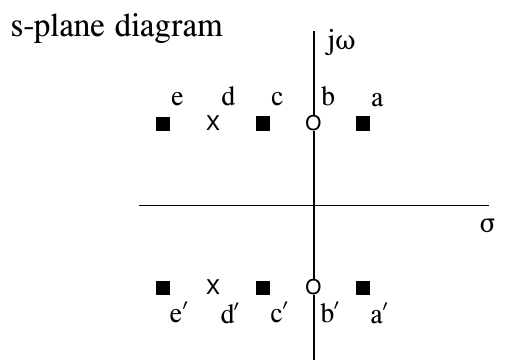
\includegraphics[width=0.425\linewidth,height=0.8\textheight,keepaspectratio]{assets/ch32/fig32-04.png}
\caption*{\textbf{图 32-4　极点-零点示例。} 这个陷波滤波器有两个极点（用 ×
表示）和两个零点（用 \dspsym{○} 表示）。这张 s
平面图标出了本例中我们要''探测''的五个位置，以分析这个系统。（图 32-5
是这个例子的继续。） （s-plane diagram = s 平面图；a～e 及 a′～e′
是五对探测位置。原书图注写的是''Figure 30-5 is a continuation''，应为图
32-5；图注原书排在左侧，裁图时已去掉。）}
\end{figure}

先考虑探测波形随时间推移幅度减小的情况，如 (a) 所示。只要 σ
\textgreater{} 0（s
平面的右半边），就会是这种情况。由于冲激响应和探测波形都随时间增加而变小，两者的乘积也有同样的特征。把两个波形的乘积从负无穷积分到正无穷，结果是某个没什么特别意义的数。特别是，一个衰减的探测波形无法抵消一个衰减的冲激响应。这意味着稳定的系统不会有
σ \textgreater{} 0 的极点。换句话说，稳定系统的所有极点都局限在 s
平面的左半边。事实上，s
平面右半边的极点表明系统是不稳定的（即冲激响应随时间增长）。

\begin{figure}[htbp]
\centering
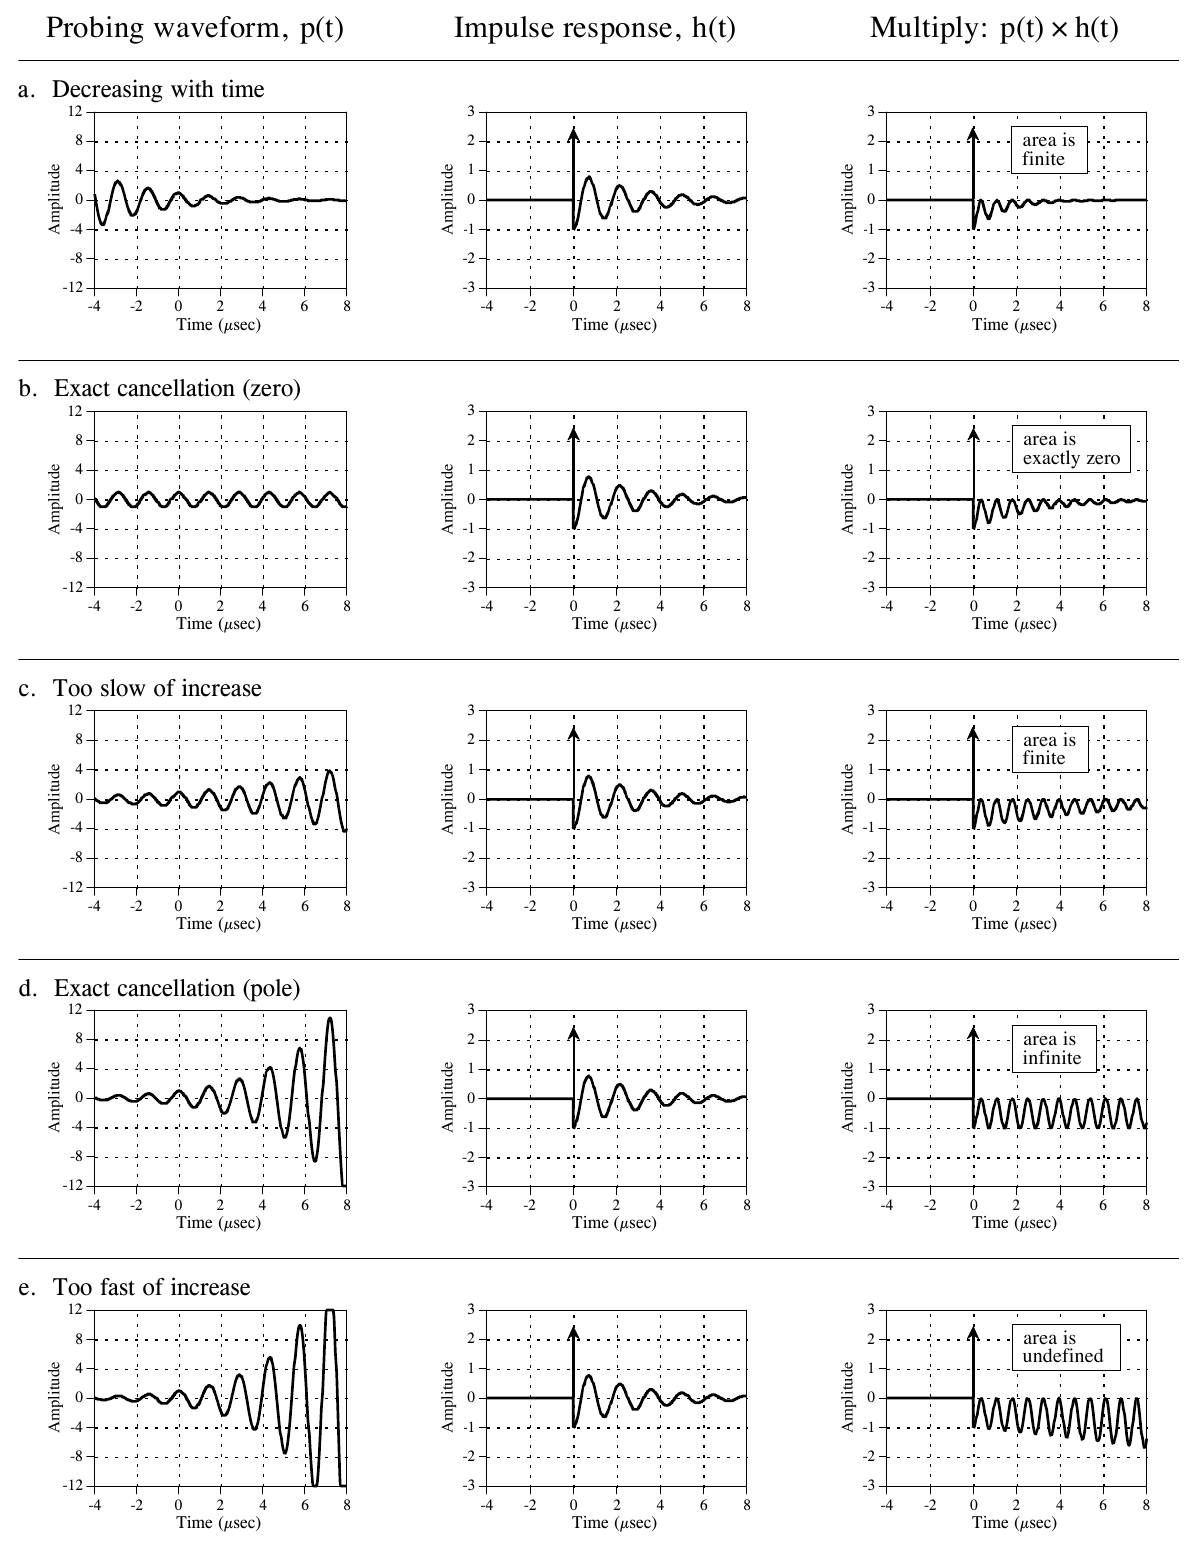
\includegraphics[width=0.988\linewidth,height=0.8\textheight,keepaspectratio]{assets/ch32/fig32-05.png}
\caption*{\textbf{图 32-5　探测冲激响应。}
拉普拉斯变换可以看作是用各种按指数衰减的正弦波去探测系统的冲激响应。能产生抵消的探测波形叫做极点和零点。本图显示五个探测波形（左栏）作用于一个陷波滤波器的冲激响应（中栏）。这五个波形在
s 平面上对应的位置见图 32-4。 （三栏依次为：Probing waveform, p(t) =
探测波形 p(t)；Impulse response, h(t) = 冲激响应 h(t)；Multiply: p(t) ×
h(t) = 相乘 p(t) × h(t)。五行依次为：a. Decreasing with time =
随时间衰减；b. Exact cancellation (zero) = 恰好抵消（零点）；c.~Too slow
of increase = 增长太慢；d.~Exact cancellation (pole) =
恰好抵消（极点）；e. Too fast of increase = 增长太快。右栏方框：area is
finite = 面积有限，area is exactly zero = 面积恰好为零，area is infinite
= 面积无穷大，area is undefined = 面积无定义。Amplitude = 幅度，Time
(µsec) = 时间（微秒）。）}
\end{figure}

\begin{enumerate}
\def\labelenumi{(\alph{enumi})}
\setcounter{enumi}{1}
\item
  是我们要找的特殊情况之一。把这个波形乘以冲激响应，得到的积分值为零。这是因为
  x 轴以上的面积（来自冲激函数）恰好等于 x
  轴以下的面积（来自经过整流的正弦波）。产生这类抵消的 σ 和 ω
  值，叫做系统的零点。如图 32-4 的 s
  平面图所示，零点用小圆圈（\dspsym{○}）表示。
\item
  是我们可以尝试的下一个探测波形。这里用的正弦波随时间按指数增长，但增长的速度慢于冲激响应随时间衰减的速度。结果两个波形的乘积也随时间推移而减小。和
  (a)
  一样，这使得乘积的积分是某个没什么意义的实数。要点在于，没有发生任何形式的恰好抵消。
\end{enumerate}

跳过一个看
(e)：这个探测波形增长的速度快于冲激响应衰减的速度。两者相乘后，得到的信号幅度随时间推移而增大。这意味着曲线下的面积随时间增加而越来越大，从
t = −\dspsym{∞} 到 +\dspsym{∞}
的总面积没有定义。用数学行话说，积分不收敛。换句话说，并不是 s
平面的所有区域都有确定的值。s
平面上积分有定义的那部分，叫收敛域(region-of-convergence)。在某些数学技术中，知道
s
平面的哪些部分在收敛域内是很重要的；不过，本书的应用不需要这个信息。本讨论只关心恰好抵消的情况。

在 (d)
中，探测波形增长的速度恰好等于冲激响应衰减的速度。这使两个波形的乘积幅度恒定。换句话说，这是
(c) 和 (e)
之间的分界线，得到的总面积''刚好没有定义''（如果数学家能原谅这种不严谨的说法的话）。更确切地说，这个点在收敛域的边界上。前面说过，产生这类恰好抵消的
σ 和 ω 值，叫做系统的极点。极点在 s 平面上用叉号（×）表示。

\section{电路分析}

我们一直用图示的方式介绍拉普拉斯变换，描述波形长什么样、怎样被处理。这是理解这种方法最直观的方式，但与它的实际用法大不相同。拉普拉斯变换本质上是一种数学技术，用法是写出公式、推演公式。问题在于，人很容易迷失在复数代数的抽象之中，失去与现实世界的一切联系。你的任务是把这两种视角融合起来。拉普拉斯变换是分析电路的主要方法。要记住，任何受微分方程支配的系统都可以用同样的方法处理，电路只是我们用的一个例子。

蛮力的做法是求解支配系统的微分方程，得到系统的冲激响应，再用公式 32-1
把冲激响应变换到 s 域。幸运的是，有一个更好的办法：把每个元件单独变换到
s 域，再考虑它们之间如何相互作用。这与第 30 章介绍的相量变换(phasor
transform)非常相似，那里电阻、电感和电容分别用 R、jωL 和 1/jωC
表示。在拉普拉斯变换中，电阻、电感和电容变成复变量 R、sL 和
1/sC。注意，相量变换是拉普拉斯变换的一个子集：在
\(s = \sigma + j\omega\) 中令 σ 为零，R 仍是 R，sL 变成 jωL，1/sC 变成
1/jωC。

和第 30
章一样，我们把三种元件各自当作一个单独的系统，电流波形是输入信号，电压波形是输出信号。说电阻、电感和电容在
s 域中变成 R、sL 和
1/sC，指的是输出除以输入。换句话说，电压波形的拉普拉斯变换除以电流波形的拉普拉斯变换，就等于这些表达式。

举个例子，设想我们强制流过电感的电流是一个幅度为 1、频率为 ω₀
的余弦波。电感两端的电压波形，可以通过求解支配它工作的微分方程得到：

\[v(t) = L\frac{d}{dt}\,i(t) = L\frac{d}{dt}\cos(\omega_0 t) = \omega_0 L \sin(\omega_0 t)\]

如果电流波形从 t = 0 开始，电压波形也从同一时刻开始（即 t \textless{} 0
时 i(t) = 0、v(t) = 0）。用公式 32-1 把这两个电压和电流波形变换到 s 域：

\[I(s) = \int_{0}^{\infty} \cos(\omega_0 t)\, e^{-st}\, dt = \frac{\omega_0}{\omega_0^2 + s^2}\]

\[V(s) = \int_{0}^{\infty} \omega_0 L \sin(\omega_0 t)\, e^{-st}\, dt = \frac{\omega_0 L s}{\omega_0^2 + s^2}\]

为了完成这个例子，我们把 s 域电压除以 s 域电流，就像用欧姆定律（R =
V/I）一样：

\[\frac{V(s)}{I(s)} = \frac{\dfrac{\omega_0 L s}{\omega_0^2 + s^2}}{\dfrac{\omega_0}{\omega_0^2 + s^2}} = sL\]

\begin{quote}
\textbf{译注：}
这个例子里正弦和余弦写反了。\(\frac{d}{dt}\cos(\omega_0 t) = -\omega_0\sin(\omega_0 t)\)，不是
\(+\omega_0\sin(\omega_0 t)\)；而
\(\int_0^\infty \cos(\omega_0 t)\,e^{-st}\,dt = s/(s^2+\omega_0^2)\)，\(\omega_0/(\omega_0^2+s^2)\)
其实是 \(\sin(\omega_0 t)\) 的拉普拉斯变换。如果把电流改成从 t = 0
开始的正弦波 \(i(t) = \sin(\omega_0 t)\)，则
\(v(t) = \omega_0 L\cos(\omega_0 t)\)，\(I(s) = \omega_0/(\omega_0^2+s^2)\)，\(V(s) = \omega_0 L s/(\omega_0^2+s^2)\)，书上两个
s 域结果和最后的 V(s)/I(s) = sL
就全部成立了。用正弦电流也恰好避开了另一个问题：余弦电流在 t = 0 从 0
跳到 1，电感电压里还会多出一个冲激 \(L\,\delta(t)\)。结论 V(s)/I(s) = sL
本身是对的。
\end{quote}

我们发现，电感两端电压的 s 域表示除以流过电感的电流的 s 域表示，等于
sL。不管我们从什么电流波形出发，结果都是如此。同样，对电阻来说，s
域电压与 s 域电流之比总是等于 R；对电容来说，总是等于 1/sC。

图 32-6 是我们要用拉普拉斯变换分析的一个示例电路，即第 30 章讨论过的 RLC
陷波滤波器。由于这种分析对所有电路都相同，我们分步骤来概述。

\textbf{第 1 步：} 把每个元件变换到 s 域。换句话说，把每个电阻的值换成
R，每个电感换成 sL，每个电容换成 1/sC。如图 32-6 所示。

\begin{figure}[htbp]
\centering
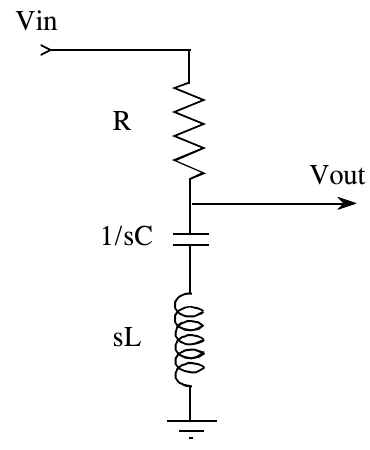
\includegraphics[width=0.308\linewidth,height=0.8\textheight,keepaspectratio]{assets/ch32/fig32-06.png}
\caption*{\textbf{图 32-6　在 s 域中分析陷波滤波器。}
这个过程的第一步，是把电阻、电感和电容的值换成它们的 s 域等效值。 （Vin
= 输入电压，Vout = 输出电压。图注原书排在左侧，裁图时已去掉。）}
\end{figure}

\textbf{第 2 步：} 求 H(s)，即输出除以输入。如第 30
章所述，做法是把每个元件都当作遵守欧姆定律，其''电阻''分别为 R、sL 和
1/sC。这样就可以使用电阻串联、电阻并联、分压器等的标准公式。把本例中的
RLC 电路当作分压器（和第 30 章一样），求得 H(s)：

\[H(s) = \frac{V_{out}(s)}{V_{in}(s)} = \frac{sL + 1/sC}{R + sL + 1/sC} = \frac{sL + 1/sC}{R + sL + 1/sC}\left[\frac{s}{s}\right] = \frac{Ls^2 + 1/C}{Ls^2 + Rs + 1/C}\]

回忆傅里叶分析中，输出信号的频谱除以输入信号的频谱，等于系统的频率响应，记作
H(ω)。上面的公式是这一概念在 s 域中的推广。信号 H(s)
叫做系统的传递函数(transfer function)，它等于输出信号的 s
域表示除以输入信号的 s 域表示。进一步说，H(s)
等于冲激响应的拉普拉斯变换，正如 H(ω) 等于冲激响应的傅里叶变换。

到目前为止，这和上一章的技术完全相同，只是用 s 代替了
jω。两种方法的区别在于此后发生的事。用 jω
只能走到这一步：我们可以画出频率响应，或者用别的方式考察它，但这在数学上是条死胡同。相比之下，拉普拉斯变换有意思的部分才刚刚开始。求出
H(s)
是拉普拉斯分析的关键，但必须把它表示成特定的形式才有用。这需要下面两步的代数变形。

\textbf{第 3 步：} 把 H(s)
整理成一个多项式除以另一个多项式。这样传递函数就写成：

\textbf{公式 32-2　多项式形式的传递函数。}

\[H(s) = \frac{a s^2 + b s + c}{a' s^2 + b' s + c'}\]

\begin{quote}
\textbf{译注：} 原书公式 32-2 的分子和分母都印成
\(as^2 + bs + c\)，从版面上看不出两组系数有区别；按后文''分子 a = L、b =
0、c = 1/C，分母 a = L、b = R、c =
1/C''的说明，分子分母是两组不同的系数，这里用带撇的 a′、b′、c′
区分分母的系数。
\end{quote}

如果系统受微分方程控制，总能把传递函数表示成这种形式。例如，图 32-3
中的矩形脉冲不是微分方程的解，它的拉普拉斯变换就不能写成这种形式。相比之下，任何由电阻、电容和电感组成的电路都可以写成这种形式。对本例中的
RLC 陷波滤波器，第 2
步中的代数运算已经把传递函数整理成了正确的形式，即：

\[H(s) = \frac{a s^2 + b s + c}{a' s^2 + b' s + c'} = \frac{Ls^2 + 1/C}{Ls^2 + Rs + 1/C}\]

其中：分子 a = L，b = 0，c = 1/C；分母 a′ = L，b′ = R，c′ = 1/C。

\textbf{第 4 步：}
对分子和分母多项式做因式分解。也就是把分子和分母多项式拆成若干个各只含一个
s
的因子，这些因子相乘必须等于原来的分子和分母。换句话说，把公式整理成如下形式：

\textbf{公式 32-3　因式分解后的 s 域。} 这种形式使 s
域可以用极点和零点来表示。

\[H(s) = \frac{(s - z_1)(s - z_2)(s - z_3)\cdots}{(s - p_1)(s - p_2)(s - p_3)\cdots}\]

分子的根 z₁, z₂, z₃, \dspsym{⋯} 是这个式子的零点，分母的根 p₁, p₂, p₃,
\dspsym{⋯}
是极点。它们就是本章前面遇到的那些零点和极点，下一节将讨论怎样使用它们。

如果分子和分母是二阶或更低阶的多项式，对 s
域表达式做因式分解很简单。换句话说，我们能轻松处理 s 和 s²
项，但处理不了 s³、s⁴、s⁵、\dspsym{⋯}。这是因为二阶多项式
\(ax^2 + bx + c\)
的根可以用求根公式求出：\(x = \left(-b \pm \sqrt{b^2 - 4ac}\right)/2a\)。用这种方法，示例陷波滤波器的传递函数可以分解为：

\[H(s) = \frac{(s - z_1)(s - z_2)}{(s - p_1)(s - p_2)}\]

其中：

\[z_1 = j/\sqrt{LC} \qquad\qquad p_1 = \frac{-R + \sqrt{R^2 - 4L/C}}{2L}\]

\[z_2 = -j/\sqrt{LC} \qquad\qquad p_2 = \frac{-R - \sqrt{R^2 - 4L/C}}{2L}\]

\begin{quote}
\textbf{译注：} 原书求根公式印作
\(x = -b \pm \sqrt{b^2 - 4ac}\ /\ 2a\)，漏了括号，按字面会读成只有根号那一项除以
2a；正确写法是 \((-b \pm \sqrt{b^2-4ac})/2a\)，上面已补上括号。
\end{quote}

和本例一样，二阶系统最多有两个零点和两个极点。系统的极点数等于独立的储能元件数。例如，电感和电容储存能量，电阻不储存。零点数等于或少于极点数。

高于二阶的多项式一般不能用代数方法分解，需要更复杂的数值方法。另一种办法是把电路构造成二阶级的级联。一个很好的例子是第
3
章介绍的那一族模拟滤波器。例如，一个八极点滤波器是由四个各含两个极点的级级联而成的。重要的是，这种多级方法是为了克服数学上的限制，而不是电子学上的限制。

\section{极点和零点的重要性}

为了让讨论不那么抽象，我们给刚才分析的陷波滤波器代入实际的元件值：R =
220 Ω，L = 54 µH，C = 470 pF。把这些值代入上面的公式，极点和零点位于：

\[z_1 = 0 + j\,6.277\times 10^6 \qquad\qquad p_1 = -2.037\times 10^6 + j\,5.937\times 10^6\]

\[z_2 = 0 - j\,6.277\times 10^6 \qquad\qquad p_2 = -2.037\times 10^6 - j\,5.937\times 10^6\]

\begin{quote}
\textbf{译注：}
我按上面的公式核算过：\(1/\sqrt{LC} = 1/\sqrt{54\times10^{-6}\times 470\times10^{-12}} \approx 6.277\times10^6\)；\(-R/2L = -220/(108\times10^{-6}) \approx -2.037\times10^6\)；\(\sqrt{4L/C - R^2}/2L \approx 5.937\times10^6\)，与原书一致。
\end{quote}

这些极点和零点的位置如图 32-7
所示。每个零点用一个圆圈表示，每个极点用一个叉号表示。这叫零极点图(pole-zero
diagram)，是显示 s 域数据最常用的方式。图 32-7 还给出了 s
平面的地形图。为简单起见，只画出了幅度，但别忘了还有相应的相位。正如山峰和山谷决定了地球表面的形状，极点和零点决定了
s
平面的形状。与山峰和山谷不同的是，每个极点和零点的形状和大小都完全相同，极点或零点唯一的独特之处就是它的位置。极点和零点之所以重要，是因为它们简洁地表示了
s
平面上任意一点的值。也就是说，我们只用几个参数就能完整描述系统的特性。对
RLC
陷波滤波器来说，只需指定四个复数参数就能表示这个系统：z₁、z₂、p₁、p₂（每个都由实部和虚部组成）。

\begin{figure}[htbp]
\centering
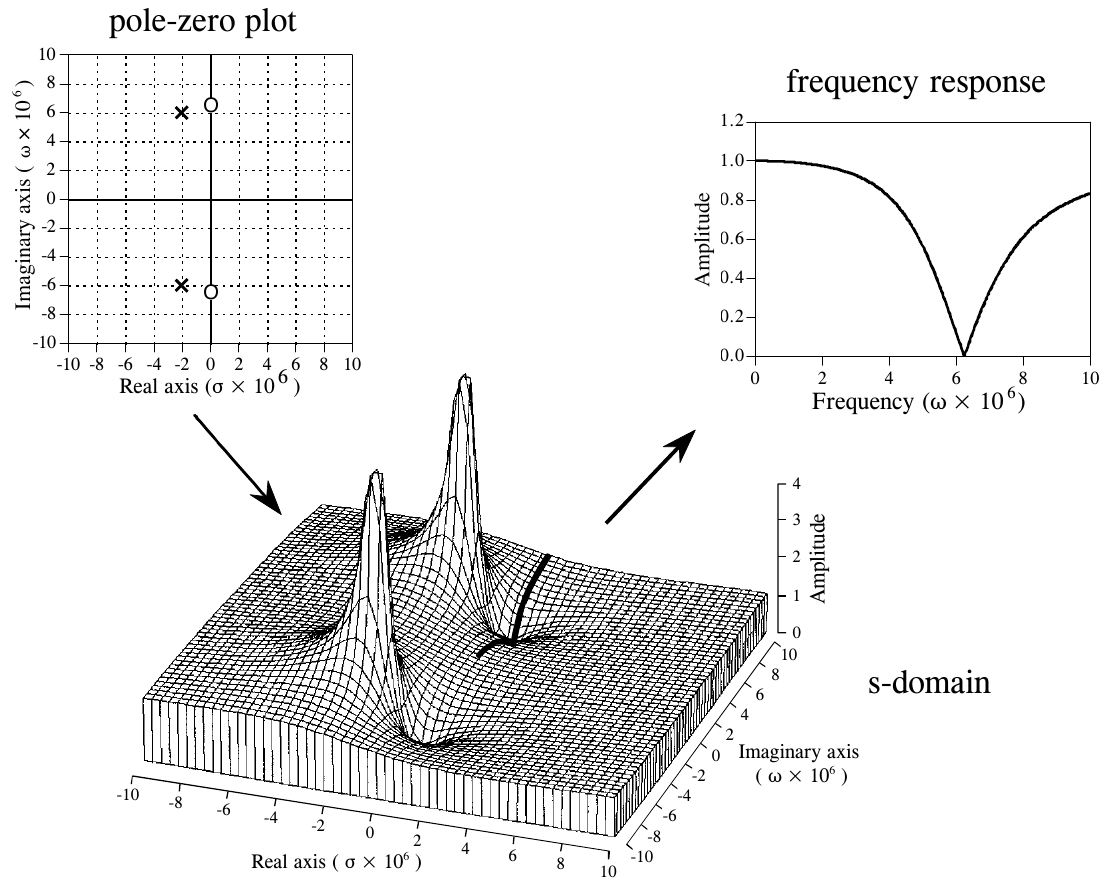
\includegraphics[width=0.925\linewidth,height=0.8\textheight,keepaspectratio]{assets/ch32/fig32-07.png}
\caption*{\textbf{图 32-7　s 域中的极点和零点。} 这几张图展示了零极点图、s
域和频率响应之间的关系。这些图中所用的陷波滤波器元件值为：R = 220 Ω，C =
470 pF，L = 54 µH。这些值把陷波中心放在 ω = 627.7 万处，即频率约为 1
MHz。 （pole-zero plot = 零极点图，frequency response =
频率响应，s-domain = s 域；Real axis (σ × 10⁶) = 实轴（σ ×
10⁶），Imaginary axis (ω × 10⁶) = 虚轴（ω × 10⁶），Frequency (ω × 10⁶) =
频率（ω × 10⁶），Amplitude =
幅度。地形图中的粗线是虚轴上的取值，即频率响应。原书 PDF 抽取时 Ω 显示为
S、p 显示为 D。）}
\end{figure}

为了更好地理解极点和零点，想象一只蚂蚁在 s
平面上爬来爬去。蚂蚁恰好所在的任何位置（即某个 s
值），都对应传递函数的一个值
H(s)。这个值是一个复数，可以表示成幅度和相位，也可以表示成实部和虚部。现在，让蚂蚁带我们到
s 平面上的一个零点去。在这个位置测得的实部和虚部都是零。这可以从公式
32-3 中 H(s) 的数学表达式理解：如果位置 s
等于任何一个零点，分子中就有一项为零，于是不管其他值是多少，整个表达式都等于零。

接下来，蚂蚁之旅把我们带到一个极点，我们再测一下 H(s)
的实部和虚部。越靠近极点的确切位置，测得的值就越大（``极点''一名正由此而来）。这同样可以从公式
32-3 理解：如果位置 s 等于任何一个
p，分母就等于零，除以零使整个表达式变成无穷大。

探索过这些特殊位置之后，蚂蚁之旅开始在 s 平面上随意游走。每个位置上 H(s)
的值完全取决于极点和零点的位置，因为这片奇特的地形里不允许有任何其他类型的特征。靠近极点，值就大；靠近零点，值就小。

公式 32-3 还描述了多个极点和零点如何相互作用，形成 s
域信号。记住，两个复数相减，得到的是它们在复平面上的距离。例如，(s − z₁)
是任意位置 s 与位于 z₁ 的零点之间的距离。因此，公式 32-3 规定：每个位置
s 上的值，等于到所有零点的距离之积，除以到所有极点的距离之积。

\begin{quote}
\textbf{译注：} 严格地说，\(s - z_1\)
是一个复数，它的模才是距离，它的辐角是方向。公式 32-3
的模等于''到各零点距离之积 ÷
到各极点距离之积''；相位则等于''各零点方向角之和 −
各极点方向角之和''。原文这里只讲了模。
\end{quote}

这就引出了本章的核心：极点和零点的位置如何让我们更深入地理解系统的频率响应。频率响应等于
H(s) 沿虚轴的值，即图 32-7
地形图中的粗线。想象蚂蚁从原点出发，沿着这条路径爬行。在原点附近，到零点的距离与到极点的距离大致相等。这使公式
32-3 的分子和分母相互抵消，在低频处给出值为 1
的频率响应。在蚂蚁接近极点和零点所在的位置之前，情况没有明显变化。接近零点时，H(s)
的值突然下降，蚂蚁正好在零点上时变为零。蚂蚁走过这对极点和零点后，H(s)
的值又恢复到
1。用这种形象化的方式可以看出，陷波的宽度取决于极点与零点之间的距离。

\begin{figure}[htbp]
\centering
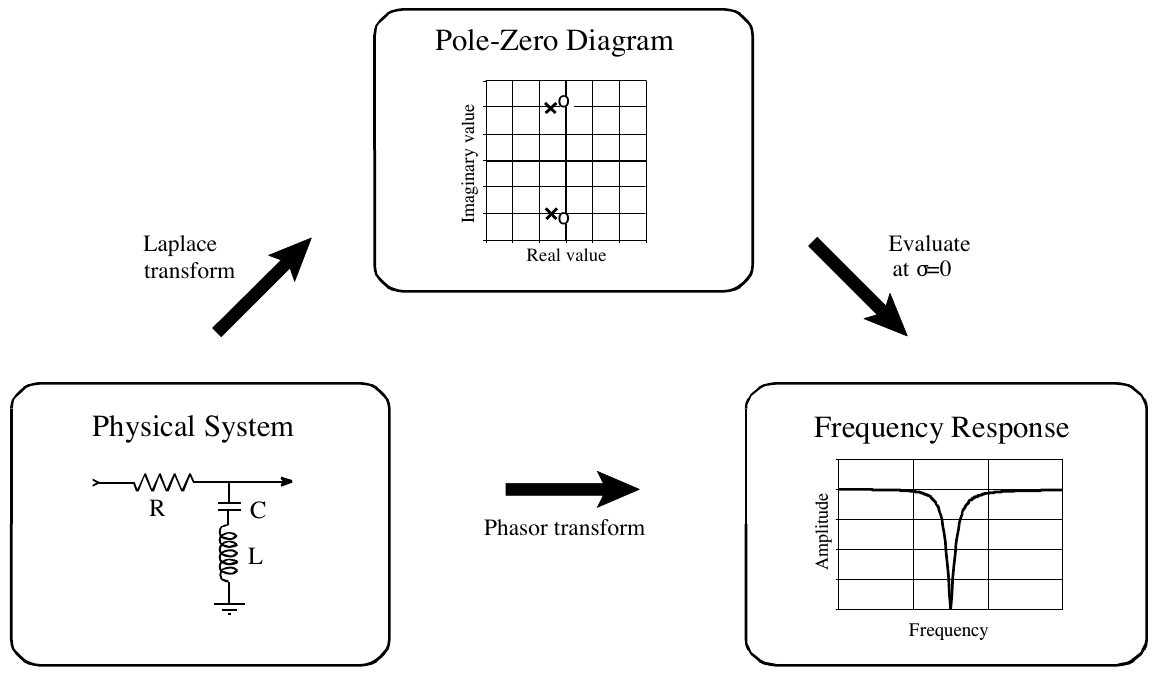
\includegraphics[width=0.963\linewidth,height=0.8\textheight,keepaspectratio]{assets/ch32/fig32-08.png}
\caption*{\textbf{图 32-8　使用拉普拉斯变换的思路。} 第 30 章介绍的相量变换（使用
R、jωL 和 −j/ωC
的方法），可以直接由物理系统的参数算出频率响应。相比之下，拉普拉斯变换从物理系统算出
s 域表示，通常以零极点图的形式显示；再由 s
域沿虚轴求传递函数的值，就得到频率响应。两种方法最终结果相同，但 s
域这个中间步骤能让我们看清频率响应为什么会这样表现。 （Physical System =
物理系统，Pole-Zero Diagram = 零极点图，Frequency Response =
频率响应；Laplace transform = 拉普拉斯变换，Evaluate at σ=0 = 在 σ = 0
处求值，Phasor transform = 相量变换；Imaginary value = 虚部值，Real
value = 实部值，Amplitude = 幅度，Frequency = 频率。）}
\end{figure}

图 32-8
总结了拉普拉斯变换的用法。我们从一个物理系统（比如一个电路）出发。如果愿意，可以像第
30
章那样，用相量变换直接得到系统的频率响应。另一种办法是用前面概述的四步法做拉普拉斯变换，得到传递函数
H(s)
的数学表达式，它可以用零极点图来表示。然后沿虚轴求传递函数的值，也就是把每个
s 都换成
jω，就得到频率响应。两种方法得到的结果相同，但作为中间步骤的零极点图让我们理解系统为什么会这样表现，以及怎样改变它。

\section{在 s 域中设计滤波器}

拉普拉斯变换最强大的应用，是直接在 s
域中设计系统。这包括两步。第一步，通过指定极点和零点的个数与位置来设计 s
域。这是一个纯数学问题，目标是得到最好的频率响应。第二步，推导出一个能提供这种
s
域表示的电子电路。这多少算一门艺术，因为能实现某个给定零极点图的电路结构有很多种。

前面说过，如果系统含有两个以上的极点或零点，拉普拉斯变换方法的第 4
步就非常困难。常见的解决办法是把多个极点和零点分到相继的若干级中去实现。例如，一个
6
极点滤波器用三个相继的级来实现，每级最多含两个极点和两个零点。由于每一级在
s
域中都可以表示为二次分子除以二次分母，这种方法叫做用双二阶节(biquad)设计。

图 32-9 是一种常见的双二阶电路，即第 3 章滤波器设计方法中用的那种。它叫
Sallen-Key 电路，得名于 R. P. Sallen 和 E. L. Key，他们在 1950
年代中期发表的一篇论文中描述了这种技术。虽然有若干种变形，最常见的电路使用两个阻值相等的电阻、两个容值相等的电容，以及一个放大倍数在
1 到 3 之间的放大器。在 Sallen 和 Key
那个年代还没有这样的条件，但现在放大器可以用低成本的运算放大器加上适当的反馈电阻来实现。按照四步电路分析法走一遍，可以把这个电路两个极点的位置与元件值联系起来：

\textbf{公式 32-4　Sallen-Key 电路的极点位置。} 这两个公式把极点位置 ω
和 σ，与放大器增益 A、电阻 R 和电容 C 联系起来。

\[\sigma = \frac{A - 3}{2RC} \qquad\qquad \omega = \frac{\pm\sqrt{-A^2 + 6A - 5}}{2RC}\]

这两个公式表明，两个极点总是位于一个半径为 1/RC
的圆上的某处。它们在圆上的确切位置取决于放大器的增益。如 (a)
所示，放大倍数为 1
时，两个极点都在实轴上。这种结构的频率响应是一个低通滤波器，通带与阻带之间的过渡比较平缓。这个电路的
−3 dB（0.707）截止频率记作 ω₀，在圆与虚轴的交点处，即 ω₀ = 1/RC。

\begin{quote}
\textbf{译注：}
可以验证这个圆：\(\sigma^2 + \omega^2 = \dfrac{(A-3)^2 + (-A^2+6A-5)}{4R^2C^2} = \dfrac{4}{4R^2C^2} = \dfrac{1}{(RC)^2}\)，与
A 无关，所以两个极点总在半径 1/RC 的圆上。A = 1 时 ω = 0、σ =
−1/RC，两个极点重合在实轴上；A = 1.586 时 σ \dspsym{≈} −0.707/RC、ω
\dspsym{≈} ±0.707/RC，正好在 45° 方向；A = 3 时 σ = 0，极点落在虚轴上。
\end{quote}

\begin{figure}[htbp]
\centering
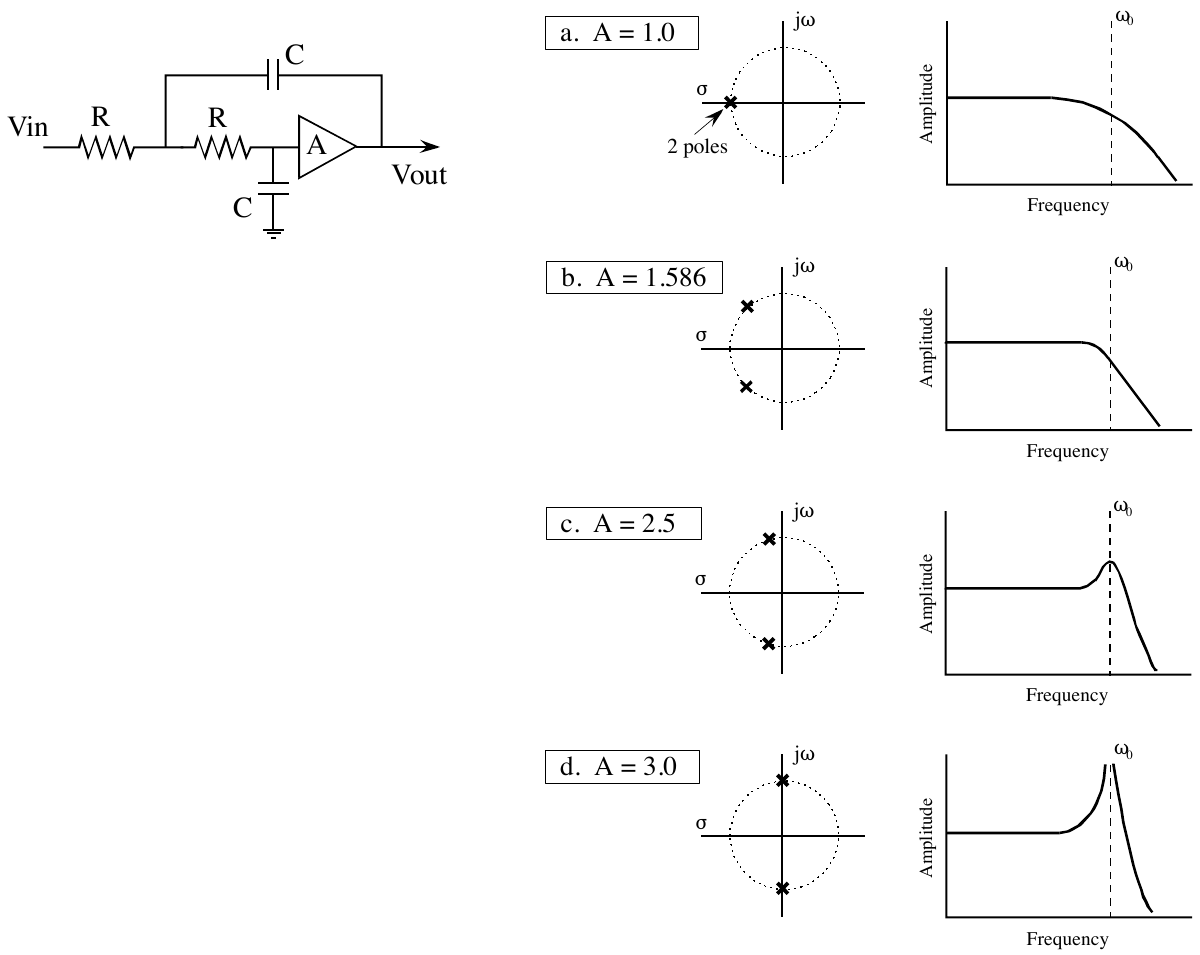
\includegraphics[width=1.000\linewidth,height=0.8\textheight,keepaspectratio]{assets/ch32/fig32-09.png}
\caption*{\textbf{图 32-9　Sallen-Key 电路的特性。} 这个电路在半径为 1/RC
的圆上产生两个极点。随着放大器增益的增加，极点从实轴（如 (a)）向虚轴（如
(d)）移动。 （左边是电路：Vin = 输入电压，Vout = 输出电压，A =
放大器。右边四行依次为 a. A = 1.0、b. A = 1.586、c.~A = 2.5、d.~A = 3.0
时的极点位置和频率响应；2 poles = 两个极点（重合），Amplitude =
幅度，Frequency = 频率，ω₀ =
截止频率。图注原书排在左侧，裁图时已去掉。）}
\end{figure}

随着放大倍数增加，极点沿着圆移动，频率响应也相应改变。如 (b)
所示，放大倍数为 1.586 时，极点位于 45°
方向，频率响应的过渡更陡。继续增大放大倍数，极点更靠近虚轴，频率响应出现峰值。(c)
表示了这种情况，放大倍数设为
2.5。随着放大倍数增大，峰值的幅度不断增长，直到增益达到 3。如 (d)
所示，这是一个特殊情况，极点正好落在虚轴上。对应的频率响应在峰值处变成无穷大。实际上，这意味着电路变成了振荡器。再增大增益，极点就被推入
s 平面的右半边更深处。前面说过，这对应于系统不稳定（自激振荡）。

以 Sallen-Key
电路为基本构件，可以构造出各种各样的滤波器。例如，把选定数量的极点均匀地放在圆的左半边上，就设计出了低通巴特沃斯滤波器(Butterworth
filter)，如图 32-10 所示。这种结构中每两个极点需要一个 Sallen-Key 级。第
3
章讲过，巴特沃斯滤波器是最平坦的，也就是说，它在频率响应不出现峰值的前提下，通带与阻带之间的过渡最陡。用的极点越多，过渡越快。由于巴特沃斯滤波器的所有极点都在同一个圆上，级联的各级都用相同的
R 和 C
值，各级之间唯一的不同是放大倍数。为什么这种圆形排列的极点能给出最平坦的响应？别去找一个显而易见或直观的答案，它就是从数学里自然得出的。

\begin{figure}[htbp]
\centering
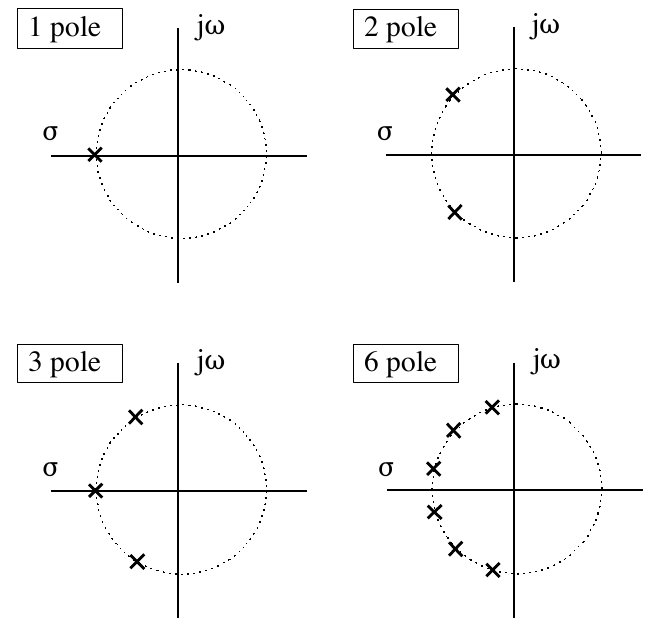
\includegraphics[width=0.542\linewidth,height=0.8\textheight,keepaspectratio]{assets/ch32/fig32-10.png}
\caption*{\textbf{图 32-10　巴特沃斯滤波器的 s 平面。}
把极点均匀地放在一个圆的左半边，就构成了低通巴特沃斯滤波器。滤波器用的极点越多，滚降越快。
（1 pole / 2 pole / 3 pole / 6 pole = 1 / 2 / 3 / 6
极点。图注原书排在左侧，裁图时已去掉。）}
\end{figure}

图 32-11
说明怎样修改巴特沃斯滤波器的极点位置，得到切比雪夫滤波器(Chebyshev
filter)。第 3
章讲过，切比雪夫滤波器以允许通带内出现纹波为代价，换取比巴特沃斯更陡的过渡。在
s
域中，这对应于把极点所在的圆压扁成一个椭圆。椭圆压得越扁，通带纹波越大，过渡也越陡。用
Sallen-Key 级的级联来构成时，各级需要不同的电阻和电容值。

图 32-11 还展示了滤波器设计思路的更高一个层次：椭圆滤波器(elliptic
filter)。椭圆滤波器允许通带和阻带都有纹波，以此实现尽可能陡的过渡。在 s
域中，这对应于把零点直接放在虚轴上，第一个零点靠近截止频率。椭圆滤波器有好几种变形，设计起来比巴特沃斯和切比雪夫结构难得多。这是因为椭圆滤波器的极点和零点不是排成简单的几何图形，而是按一种涉及椭圆函数和椭圆积分的数学方式排列的（名字正由此而来）。

\begin{quote}
\textbf{译注：} 原文说椭圆滤波器''把零点直接放在实轴上(real
axis)``，应为虚轴(imaginary axis)。图 32-11
中椭圆滤波器的零点（\dspsym{○}）画在 jω
轴上；零点在虚轴上，频率响应才会在对应频率处降到零，形成阻带中的那些凹口。
\end{quote}

\begin{figure}[htbp]
\centering
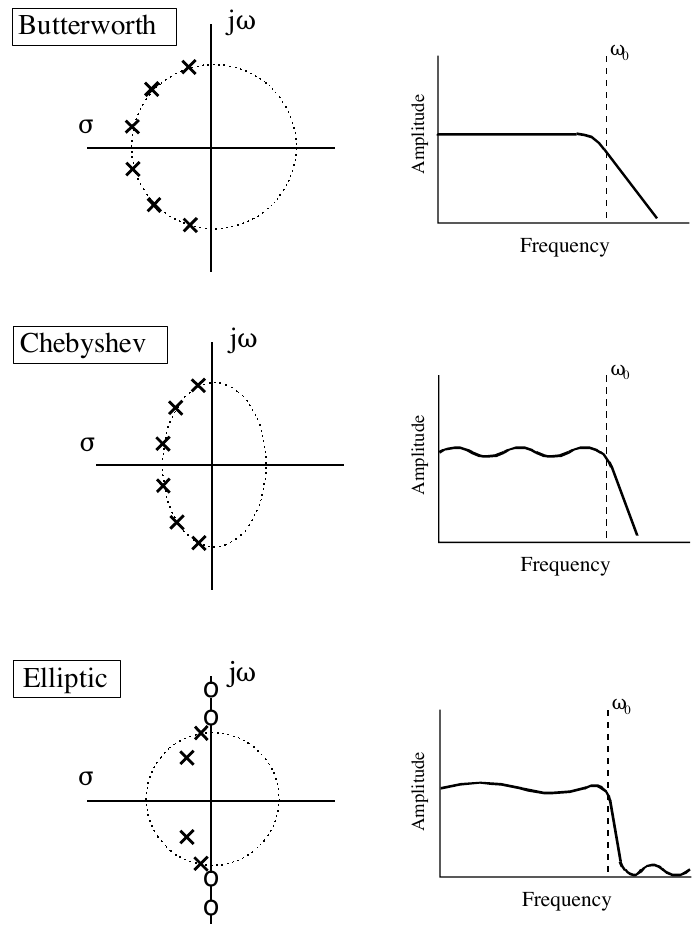
\includegraphics[width=0.579\linewidth,height=0.8\textheight,keepaspectratio]{assets/ch32/fig32-11.png}
\caption*{\textbf{图 32-11　经典的零极点图样。}
这是滤波器设计中三种经典的零极点图样。巴特沃斯滤波器的极点在一个圆上等间隔排列，得到最平坦的响应。切比雪夫滤波器的极点放在一个椭圆上，过渡更陡，但代价是通带内有纹波。椭圆滤波器在阻带中加入零点，过渡更快，但通带和阻带都有纹波。
（Butterworth = 巴特沃斯，Chebyshev = 切比雪夫，Elliptic =
椭圆；Amplitude = 幅度，Frequency = 频率，ω₀ =
截止频率。图注原书排在左侧，裁图时已去掉。）}
\end{figure}

由于每个双二阶节产生两个极点，偶数阶滤波器（2 极点、4 极点、6
极点等）可以用双二阶节级联构成。然而，奇数阶滤波器（1 极点、3 极点、5
极点等）需要一样双二阶节提供不了的东西：实轴上的单个极点。这只不过是在级联中加一个简单的
RC 电路。例如，一个 9 极点滤波器可以由 5 级构成：4 个 Sallen-Key
双二阶节，再加一级由一个电容和一个电阻组成的电路。

\begin{quote}
\textbf{译注：} 原文说奇数阶滤波器需要''虚轴上(imaginary
axis)的单个极点''，应为实轴(real axis)。单个实极点才对应一个实际的 RC
电路；看图 32-10 的 1 极点和 3
极点，那个单独的极点都在负实轴上。译文已按实轴翻译。
\end{quote}

这些经典的零极点图样都是针对低通滤波器的，但可以修改成其他频率响应。做法是先设计一个低通滤波器，再在
s 域中做一个数学变换。我们先算出低通滤波器的极点位置，把传递函数 H(s)
写成公式 32-3 的形式。把每个''s''都换成''1/s''，再把式子重新整理成公式
32-3
的零极点形式，就得到相应的高通滤波器的传递函数。这样就定义了实现高通滤波器的新极点和零点位置。更复杂的
s 域变换可以从最初的低通设计得到带通和带阻滤波器。这类 s
域中的数学处理是滤波器设计的中心议题，有整本整本的书专门讨论它。模拟滤波器设计是
90\% 的数学加 10\% 的电子学。

幸运的是，用 Sallen-Key 级设计高通滤波器不需要这种数学处理。s
域中用''1/s''替换''s''，对应于把电路中的电阻和电容互换。在 s
平面上，这种互换把极点放到新的位置，并在原点处直接加上两个零点。这使频率响应在直流（零频率）处的值为零，正如高通滤波器所应有的。这就让
Sallen-Key 电路发挥出全部潜力：实现两个极点和两个零点。
